% !TeX root = er.tex


\chapter{Comportement réactif}\label{ch.reactive}

Nous sommes maintenant prêts à écrire nos premiers algorithmes pour les robots. Ces algorithmes démontrent un \emph{comportement réactif}\index{comportement réactif} : un événement (tel que la détection d'un objet proche par le robot) amène le robot à réagir en effectuant une action qui modifie son comportement (comme l'arrêt des moteurs). On parle de comportement purement réactif lorsque l'action est liée uniquement à l'occurrence d'un événement et ne dépend pas des données stockées en mémoire (état).

Les comportements réactifs sont ceux des \emph{véhicules de Braitenberg} qui sont appropriés pour introduire la robotique car un comportement complexe découle d'algorithmes simples. Les sections~\ref{s.braitenberg} à \ref{s.turning} décrivent les véhicules de Braitenberg qui ont un comportement réactif ; dans le chapitre~\ref{ch.fmg} nous présentons les véhicules de Braitenberg qui ont un comportement non réactif avec des états. La section~\ref{s.line} présente plusieurs algorithmes pour le comportement réactif classique du suivi de ligne. Le suivi de ligne est une tâche intéressante car les algorithmes sont sensibles aux caractéristiques des capteurs et des lignes. Une calibration est nécessaire pour déterminer les seuils optimaux pour un mouvement rapide et robuste du robot. La section ~\ref{s.abstract-vehicles} donne un bref aperçu de la formulation originale des véhicules de Braitenberg dans une approche biologique avec des capteurs connectés directement aux moteurs, et non à travers un ordinateur. Plus loin dans le livre (Sect.~\ref{s.braitenberg-ann}) nous discutons de l'implémentation des véhicules de Braitenberg en utilisant des réseaux de neurones.

\section{Véhicules Braitenberg}\label{s.braitenberg}
\index{Véhicule Braitenberg}

Valentino Braitenberg est un neuroscientifique qui a décrit la conception de véhicules virtuels présentant un comportement étonnamment complexe. Des chercheurs du MIT Media Lab ont développé des implémentations matérielles de ces véhicules à partir de \emph{briques programmables} qui étaient les précurseurs des \lego{}. Mindstorms.\footnote{Le rapport du MIT utilise le terme \emph{créatures de Braitenberg} mais nous conservons le terme original.} Ce chapitre décrit une implémentation de la plupart des véhicules Braitenberg du rapport du MIT. Le matériel du MIT utilisait des capteurs de lumière et de toucher, alors que notre robot générique est basé sur des capteurs de proximité horizontaux.

Pour faciliter la comparaison avec le rapport du MIT (et indirectement avec le livre de Braitenberg), les noms de leurs véhicules ont été conservés, même s'il peut être difficile de comprendre leur signification dans nos implémentations.

Deux véhicules sont présentés en détail en donnant tout ce qui suit :
\begin{itemize}
\item La spécification du comportement du robot ;
\item Un algorithme formalisé pour le comportement spécifié ;
\item Une activité qui vous demande d'implémenter l'algorithme sur votre robot.
\end{itemize}
Les autres véhicules sont présentés dans des activités qui spécifient le comportement et vous demandent de développer un algorithme et de l'implémenter sur votre robot.

\section{Réaction à la détection d'un objet}\label{s.reacting}

\begin{quote}
\normalsize\noindent{}\textbf{Spécification (Timid):}\index{Véhicule Braitenberg!timid} Lorsque le robot ne détecte pas d'objet, il se déplace vers l'avant. Lorsqu'il détecte un objet, il s'arrête.
\end{quote}

\noindent{} L'algorithme~\ref{alg.timid} implémente ce comportement.

\begin{figure}
\begin{alg}{Timide}{timid}
\hline
\stl{}&when object not detected in front&\\
\stl{}&\idc{} left-motor-power \ass $100$&\\
\stl{}&\idc{} right-motor-power \ass $100$&\\
\stl{}&&\\
\stl{}&when object detected in front&\\
\stl{}&\idc{} left-motor-power \ass $0$&\\
\stl{}&\idc{} right-motor-power \ass $0$&\\
\end{alg}
\end{figure}

L'algorithme utilise deux gestionnaires d'événements, un pour l'événement de détection d'un objet et un pour l'événement de non-détection d'un objet. Les gestionnaires d'événements sont écrits en utilisant l'instruction \p{when} dont la signification est :

\begin{center}
\p{lorsque l'événement \emph{premier} se produit, effectuez les actions suivantes}.
\end{center}
\noindent{}Pourquoi utilisons-nous cette construction et non l'instruction \p{while} plus familière (Algorithme~\ref{alg.timid-a}) ?

\begin{figure}
\begin{alg}{Timide avec while}{timid-a}
\hline
\stl{}&while object not detected in front&\\
\stl{}&\idc{} left-motor-power \ass $100$&\\
\stl{}&\idc{} right-motor-power \ass $100$&\\
\stl{}&&\\
\stl{}&while object detected in front&\\
\stl{}&\idc{} left-motor-power \ass $0$&\\
\stl{}&\idc{} right-motor-power \ass $0$&\\
\end{alg}
\end{figure}

Si l'on utilise l'instruction \p{while}, \emph{as tant} que l'objet n'est pas détecté, les moteurs sont activés, et \emph{ tant} que l'objet est détecté, les moteurs sont désactivés. Comme le capteur détectera l'objet sur une certaine distance, les moteurs seront activés ou désactivés à plusieurs reprises. Il est probable qu'aucun dommage ne sera causé si un moteur déjà éteint est éteint et un moteur déjà allumé est allumé, mais ces commandes répétées ne sont pas nécessaires et peuvent gaspiller des ressources. Par conséquent, nous préférons éteindre les moteurs uniquement lorsque l'objet est détecté pour la première fois et les allumer uniquement lorsque l'objet n'est pas détecté pour la première fois. L'instruction \p{when} donne la sémantique que nous souhaitons.

\begin{framed}
\act{Timide}{timid}
\begin{itemize}
\item Implémente le comportement Timide.
\end{itemize}
\end{framed}

\begin{framed}
\act{Indécisif}{indécisif}
\begin{itemize}
\item Implémente le comportement Indécis.
\begin{quote}
\normalsize\noindent\textbf{Spécification (Indécis)~:~}Lorsque le robot ne détecte pas d'objet, il se déplace vers l'avant. Lorsqu'il détecte un objet, il recule.
\end{quote}
\item A la bonne distance, le robot va \emph{osciller}, c'est-à-dire qu'il va avancer et reculer en succession rapide. Mesurez cette distance pour votre robot et pour des objets de réflectivité différente.
\end{itemize}
\end{framed}

\begin{framed}
\act{Dogged}{dogged}
\begin{itemize}
\item Implémente le comportement Dogged.
\begin{quote}
\normalsize\noindent\textbf{Spécification (Dogged)~:~}Lorsque le robot détecte un objet à l'avant, il recule. Lorsque le robot détecte un objet à l'arrière, il se déplace vers l'avant.
\end{quote}
\end{itemize}
\end{framed}

\begin{framed}
\act{Dogged (arrêt)}{dogged1}
\begin{itemize}
\item Implémente le comportement Dogged (arrêt).
\begin{quote}
\normalsize\noindent\textbf{Spécification (Dogged (arrêt))~:~} Comme dans Activity~\ref{act.dogged}, mais lorsqu'un objet n'est pas détecté, le robot s'arrête.
\end{quote}
\end{itemize}
\end{framed}

\begin{framed}
\act{Attractive et répulsive}{attractive}
\begin{itemize}
\item Met en oeuvre le comportement Attractif et repoussant.
\begin{quote}
\normalsize\noindent\textbf{Spécification (Attraction et répulsion)~:~} Lorsqu'un objet s'approche du robot par derrière, le robot s'enfuit jusqu'à ce qu'il soit hors de portée.
\end{quote}
\end{itemize}
\end{framed}


\section{Réaction et virage}\label{s.turning}

Une voiture tourne en modifiant l'angle de ses roues avant par rapport au châssis du véhicule. La puissance du moteur n'est pas modifiée. Un robot à entraînement différentiel ne possède pas de mécanisme de direction (comme le volant d'une voiture ou le guidon d'un vélo). Au lieu de cela, il tourne en réglant différents niveaux de puissance sur les roues gauche et droite. Si une roue tourne plus vite que l'autre, le robot tourne dans la direction opposée à celle de la roue la plus rapide (Fig.\ref{fig.left-gentle}). Si une roue tourne en arrière tandis que l'autre tourne en avant, le virage est beaucoup plus serré (Fig.~\ref{fig.left-sharp}). Sur les figures, les flèches indiquent la direction et la vitesse de chaque roue. Le \emph{rayon de virage}\index{rayon de virage} est le rayon du cercle qui constitue la trajectoire du robot. On dit qu'un virage est plus serré si le rayon est plus petit. À l'extrême, si une roue tourne en avant et la seconde en arrière à la même vitesse, le robot tourne sur place et le rayon de braquage est nul.

\begin{figure}
\begin{minipage}{.45\textwidth}
\begin{tikzpicture}
\pic[rotate=10,scale=1.2] at (0,0) { robot };
\draw[raxis] (0,0mm) -- (-80:15mm);
\draw[raxis] (0,0mm) -- (100:15mm);
\draw[raxis] (0,0) -- (10:8pt);
\draw[raxis] (0,0) -- (190:8pt);
\draw[->] (6mm,-8.5mm) -- +(10:15mm);
\draw[->] (3mm,10.3mm) -- +(10:5mm);
\end{tikzpicture}
\caption{Tourner doucement à gauche}\label{fig.left-gentle}
\end{minipage}
\hspace{\fill}
\begin{minipage}{.45\textwidth}
\begin{tikzpicture}
\pic[rotate=45,scale=1.2] at (0,0) { robot };
\draw[raxis] (0,0mm) -- (-45:15mm);
\draw[raxis] (0,0mm) -- (135:15mm);
\draw[raxis] (0,0) -- (45:8pt);
\draw[raxis] (0,0) -- (225:8pt);
\draw[->] (9.6mm,-3.6mm) -- +(45:15mm);
\draw[->] (-9.5mm,3.7mm) -- +(-135:5mm);
\end{tikzpicture}
\caption{Virage brusque à gauche}\label{fig.left-sharp}
\end{minipage}
\end{figure}

Implémentons maintenant un véhicule de Braitenberg dont la spécification impose au robot de tourner.

\begin{quote}
\normalsize\noindent\textbf{Spécification (Paranoïde):}\index{Véhicule de Braitenberg!paranoid} Lorsque le robot détecte un objet, il se déplace vers l'avant (en entrant en collision avec l'objet). Lorsqu'il ne détecte pas d'objet, il se tourne vers la gauche.
\end{quote}
L'algorithme~\ref{alg.paranoid} met en œuvre ce comportement.

\medskip

\begin{alg}{Paranoïde}{paranoid}
\hline
\stl{}&when both sensors detect black&\\
\stl{}&\idc{} left-motor-power \ass $100$&\\
\stl{}&\idc{} right-motor-power \ass $100$&\\
\stl{}&&\\
\stl{}&when neither sensor detects black&\\
\stl{}&\idc{} left-motor-power \ass $0$&\\
\stl{}&\idc{} right-motor-power \ass $0$&\\
\stl{}&&\\
\stl{}&when only the left sensor detects black&\\
\stl{}&\idc{} left-motor-power \ass $0$&\\
\stl{}&\idc{} right-motor-power \ass $50$&\\
\stl{}&&\\
\stl{}&when only the right sensor detects black&\\
\stl{}&\idc{} left-motor-power \ass $50$&\\
\stl{}&\idc{} right-motor-power \ass $0$&\\
\end{alg}

\begin{framed}
\act{Paranoïde}{paranoïde}
\begin{itemize}
\item Implémente le comportement Paranoïde.
\item Dans l'algorithme, les moteurs gauche et droit sont réglés sur des puissances égales mais opposées. Expérimentez ces niveaux de puissance pour voir leur influence sur le rayon de braquage du robot.
\end{itemize}
\end{framed}

\begin{framed}
\act{Paranoïde (droite-gauche)}{paranoïde1}
\begin{itemize}
\item Implémente le comportement Paranoïaque (droite-gauche).
\begin{quote}
\normalsize\noindent\textbf{Spécification (Paranoïaque (droite-gauche)):}\index{Véhicule Braitenberg!paranoïaque} Lorsqu'un objet est détecté devant le robot, ce dernier se déplace vers l'avant. Lorsqu'un objet est détecté à droite du robot, ce dernier tourne à droite. Lorsqu'un objet est détecté à la gauche du robot, le robot tourne à gauche. Lorsqu'aucun objet n'est détecté, le robot ne bouge pas.
\end{quote}
\end{itemize}
\end{framed}

\begin{framed}
\act{Insécurité}{insecure}
\begin{itemize}
\item Implémente le comportement de Insécurité.
\begin{quote}
\normalsize\noindent\textbf{Spécification (Insécurité):}\index{Véhicule Braitenberg!insecure} Si aucun objet n'est détecté à gauche du robot, réglez le moteur droit pour qu'il tourne vers l'avant et désactivez le moteur gauche. Si un objet est détecté à gauche du robot, désactivez le moteur droit et désactivez le moteur gauche pour qu'il tourne vers l'avant.
\end{quote}
\item Expérimentez avec les paramètres du moteur jusqu'à ce que le robot suive un mur sur sa gauche.
\end{itemize}
\end{framed}

\begin{framed}
\act{Conduite}{driven} (action entraînée)
\begin{itemize}
\item Implémente le comportement Conduite.
\begin{quote}
\normalsize\noindent\textbf{Spécification (Conduite):}\index{Véhicule Braitenberg!driven} Si un objet est détecté à gauche du robot, réglez le moteur droit pour qu'il tourne vers l'avant et désactivez le moteur gauche. Si un objet est détecté à droite du robot, désactivez le moteur droit et désactivez le moteur gauche pour qu'il tourne vers l'avant.
\end{quote}
\item Expérimentez les paramètres du moteur jusqu'à ce que le robot s'approche de l'objet en zigzag.
\end{itemize}
\end{framed}


\section{Ligne suivante}\label{s.line}
\index{ligne suivante}

Considérons un entrepôt équipé de chariots robotisés qui apportent des objets à une zone de distribution centrale (\ref{fig.warehouse}). Des lignes sont peintes sur le sol de l'entrepôt et le robot a pour instruction de suivre ces lignes jusqu'à ce qu'il atteigne l'emplacement de l'objet désiré.

\begin{figure}
\begin{center}
\begin{tikzpicture}[thick, rounded corners, shelf/.style={draw, minimum height=1.2cm, rectangle split, rectangle split parts=2}]
\draw  (-.8,2.0) -- (-.8,1.7) -- (2.2,1.7) -- (2.2,0) -- (3.6,0) -- (3.6,1.7) -- (5.0,1.7) -- (5.0,0) -- (6.6,0) -- (6.6,2.8) -- (-.8,2.8) -- (-.8,2.6);
\node[draw, shape=rectangle, minimum height=1pt] at (-.8,2.3) {\textsf{Envoi}};
\node[shelf] at (1.5,.8) {\textsf{A}\nodepart{two}\textsf{B}};
\node[shelf] at (2.9,.8) {\textsf{C}\nodepart{two}\textsf{D}};
\node[shelf] at (4.3,.8) {\textsf{E}\nodepart{two}\textsf{F}};
\node[shelf] at (5.7,.8) {\textsf{G}\nodepart{two}\textsf{H}};
\end{tikzpicture}
\caption{Un entrepôt robotisé}\label{fig.warehouse}
\end{center}
\end{figure}

Le \emph{suivi de ligne} est une tâche qui fait ressortir toute l'incertitude de la construction de robots dans le monde réel. La ligne peut ne pas être parfaitement droite, la poussière peut masquer une partie de la ligne ou une roue peut se déplacer plus lentement que l'autre à cause de la poussière. Pour suivre une ligne, le robot doit décider s'il est sur la ligne ou non, et s'il commence à quitter la ligne d'un côté, il doit tourner dans la bonne direction pour regagner la ligne.


\subsection{Suivi de ligne avec une paire de capteurs au sol}

Pour suivre une ligne, il est possible d'utiliser une paire de capteurs au sol (Fig. ~\ref{fig.ground-on-a-line}).\footnote{La figure montre une vue de dessus bien que les capteurs au sol se trouvent en bas du robot. Un capteur de sol sur un sol clair détectera beaucoup de lumière réfléchie. Si une ligne sombre est peinte sur le sol, le capteur détectera très peu de lumière réfléchie lorsqu'il se trouvera au-dessus de la ligne. Si votre sol est de couleur foncée, vous devez utiliser une ligne blanche.} La ligne doit être noire pour augmenter le contraste avec le sol blanc, mais la figure affiche la ligne en gris clair afin de ne pas masquer le robot et ses capteurs. Des seuils sont utilisés pour déterminer le moment où un capteur passe de la détection de la ligne à la détection du sol ou inversement.

\begin{figure}
\begin{center}
\begin{tikzpicture}[scale=1.1]
\draw [fill,lightgray] (-2,-3.5mm) rectangle +(7,8mm) ;
\pic at (0,0) { robot2 } ;
\end{tikzpicture}
\caption{Un robot avec deux capteurs de sol sur une ligne}\label{fig.ground-on-a-line}
\end{center}
\end{figure}

La ligne doit être suffisamment large pour que les deux capteurs de sol détectent l'obscurité lorsque le robot se trouve directement au-dessus de la ligne. Il n'est pas nécessaire que les capteurs soient entièrement au-dessus de la ligne ; il suffit que la quantité de lumière réfléchie par la ligne sur le capteur soit inférieure au seuil défini pour le noir.

Pour mettre en œuvre le suivi de ligne, le robot doit avancer chaque fois que les deux capteurs détectent une surface sombre, indiquant qu'il se trouve sur la ligne. Si le robot commence à quitter la ligne, le capteur de sol gauche ou droit quittera la ligne en premier (Fig.\ref{fig.leave-left-right}) :

\begin{figure}
\begin{center}
\begin{tikzpicture}[scale=1.1]
\draw[fill,lightgray] (-1,-3.5mm) rectangle +(7,8mm);
\pic[rotate=10] at (0,3mm) { robot2 };
\pic[rotate=-10] at (4,-3mm) { robot2 };
\end{tikzpicture}
\caption{Quitter la ligne}\label{fig.leave-left-right}
\end{center}
\end{figure}

\begin{itemize}
\item Si le robot sort de la ligne vers le \emph{gauche}, le capteur du \emph{gauche} ne détectera pas la ligne alors que le capteur du \emph{droite} la détecte toujours ; le robot doit tourner vers le \emph{droite}.
\item Si le robot sort de la ligne vers la \emph{droite}, le capteur de \emph{droite} ne détectera pas la ligne tant que le capteur de \emph{gauche} la détecte encore ; le robot doit tourner vers la \emph{gauche}.
\end{itemize}
Pour l'instant, nous spécifions que le robot s'arrête dès qu'aucun des deux capteurs ne détecte la ligne.

L'algorithme~\ref{alg.line-two} formalise la description informelle ci-dessus.

\begin{figure}
\begin{alg}{Suivi de ligne avec deux capteurs}{line-two}
\hline
&\idv{}integer black-threshold \ass 20&\\
&\idv{}integer white-threshold \ass 80&\\
\hline
\stl{}&when black-threshold $\leq$ sensor value $\leq$ white-threshold&\\
\stl{}&\idc{} left-motor-power \ass $100$&\\
\stl{}&\idc{} right-motor-power \ass $100$&\\
\stl{}&&\\
\stl{}&when sensor value $>$ white-threshold&\\
\stl{}&\idc{} left-motor-power \ass $-50$&\\
\stl{}&\idc{} right-motor-power \ass $50$&\\
\stl{}&&\\
\stl{}&when black-threshold $<$ sensor value&\\
\stl{}&\idc{} left-motor-power \ass $50$&\\
\stl{}&\idc{} right-motor-power \ass $-50$&\\
\end{alg}
\end{figure}

\begin{framed}
\act{Suivi de ligne avec deux capteurs}{suivi de ligne-un}
\begin{itemize}
\item Implémentation de l'algorithme~\ref{alg.line-two}.
\item Utilisez du ruban adhésif noir d'électricien ou du ruban adhésif à gaffer pour créer une ligne sur le sol. (Le ruban adhésif à gaffer est utilisé sur les plateaux de théâtre et de cinéma pour attacher les câbles ou les fixer au sol. Le ruban de gaffer est généralement moins réfléchissant que le ruban d'électricien et constitue donc un meilleur choix pour la mise en œuvre d'algorithmes de suivi de ligne).
\item La ligne doit présenter des angles ou des courbes qui amèneront le robot à sortir de la ligne. Exécutez le programme et vérifiez que le robot peut suivre la ligne avec ses angles et ses courbes.
\item Expérimentez la puissance des moteurs pour revenir sur la ligne. Si le virage est trop doux, l'autre capteur risque de sortir de la ligne avant que le robot ne fasse demi-tour. Si le virage est trop serré, le robot risque de sortir de l'autre côté de la ligne. Dans tous les cas, les virages serrés peuvent être dangereux pour le robot et provoquer la chute de ce qu'il transporte.
\item La vitesse d'avancement du robot sur la ligne est également importante. Si elle est trop rapide, le robot peut sortir de la ligne avant que les virages n'affectent sa direction. Si la vitesse est trop lente, personne n'achètera votre robot pour l'utiliser dans un entrepôt. À quelle vitesse votre robot peut-il suivre la ligne sans la quitter ?
\end{itemize}
\end{framed}

\begin{framed}
\act{Différentes configurations de ligne}{line-config}
\begin{itemize}
\item Quel est le virage le plus serré que votre robot peut suivre ? Peut-il suivre une ligne qui a un virage de $90^\circ$ ?
\item Expérimentez différentes configurations de la ligne : virages doux, virages serrés et lignes en zigzag.
\item Faites des expériences avec la largeur de la ligne. Que se passe-t-il si la ligne est beaucoup plus large ou plus étroite que la distance entre les capteurs ?
\end{itemize}
\end{framed}

\begin{framed}
\act{Reprendre la ligne après l'avoir perdue}{regaining}
\begin{itemize}
\item Modifiez l'algorithme pour que le robot retourne sur la ligne après l'avoir perdue, c'est-à-dire lorsque les deux capteurs ne détectent plus de noir.
\item Algorithme 1 : avant que les deux capteurs ne détectent plus la ligne, l'un d'eux sera le premier à ne plus détecter la ligne. Utilisez une variable pour vous souvenir du capteur qui a perdu la ligne en premier ; lorsque la ligne est perdue, tournez dans la direction opposée à la valeur de cette variable.
\item Algorithme 2 : l'algorithme précédent peut ne pas fonctionner si le robot se déplace trop rapidement et sort de la ligne avant de détecter qu'un seul capteur a perdu la ligne. Au lieu de cela, si les deux capteurs ne détectent plus de noir, faites en sorte que le robot recherche la ligne sur une courte distance, d'abord dans une direction, puis dans l'autre.
\end{itemize}
\end{framed}

\begin{framed}
\act{Configuration du capteur}{sensor-config}
\begin{itemize}
\item Discutez de l'effet que les modifications suivantes apportées au robot auraient sur sa capacité à suivre une ligne :
\begin{itemize}
\item Les événements de détection du sol se produisent plus souvent ou moins souvent.
\item Les capteurs sont plus éloignés ou plus proches les uns des autres.
\item Il y a plus de deux capteurs de sol sur la partie inférieure du robot.
\item Les capteurs sont situés à l'arrière du robot ou le robot se déplace en arrière.
\end{itemize}
\item Expérimentez ces changements s'ils peuvent être effectués sur votre robot.
\end{itemize}
\end{framed}

\subsection{Suivi de ligne avec un seul capteur au sol}

Un robot peut suivre une ligne avec un seul capteur au sol si la réflectivité de la ligne varie sur sa largeur. La figure~\ref{fig.gradient} montre une ligne en niveaux de gris dont la teinte varie continuellement du noir au blanc sur toute sa largeur. Le capteur de sol renvoie des valeurs comprises entre $0$ et $100$ en fonction de la partie de la ligne sur laquelle il se trouve.

\begin{figure}
\begin{center}
\begin{tikzpicture}[scale=1.1]
\shadedraw[top color=black, bottom color = white] (-2,-3.5mm) rectangle +(7,8mm);
\pic at (0,0) { robot1 };
\end{tikzpicture}
\caption{Une ligne avec un dégradé de gris}\label{fig.gradient}
\end{center}
\end{figure}

Lorsque le robot se trouve directement au-dessus du centre de la ligne, le capteur renvoie la valeur $50$ qui se situe à mi-chemin entre le noir et le blanc. Bien sûr, nous ne nous attendons pas à ce que la valeur soit exactement $50$, il n'y a donc aucune raison pour que le robot tourne à gauche ou à droite à moins que la valeur ne s'approche de $0$ ou $100$. Nous définissons deux seuils :
\begin{itemize}
\item \p{seuil noir} : en dessous de cette valeur, le robot quitte le côté gauche de la ligne.
\item \p{seuil blanc} : au-dessus de cette valeur, le robot quitte le côté droit de la ligne.
\end{itemize}
L'algorithme~\ref{alg.line-one} modifie les paramètres de puissance du moteur lorsque la valeur renvoyée par le capteur franchit les seuils.

\begin{figure}
\begin{alg}{Suivi de ligne avec un capteur}{line-one}
&\idv{}integer black-threshold \ass 20&\\
&\idv{}integer white-threshold \ass 80&\\
\hline
\stl{}&when black-threshold $\leq$ sensor value $\leq$ white-threshold&\\
\stl{}&\idc{} left-motor-power \ass $100$&\\
\stl{}&\idc{} right-motor-power \ass $100$&\\
\stl{}&&\\
\stl{}&when sensor value $>$ white-threshold&\\
\stl{}&\idc{} left-motor-power \ass $-50$&\\
\stl{}&\idc{} right-motor-power \ass $50$&\\
\stl{}&&\\
\stl{}&when black-threshold $<$ sensor value&\\
\stl{}&\idc{} left-motor-power \ass $50$&\\
\stl{}&\idc{} right-motor-power \ass $-50$&\\
\end{alg}
\end{figure}

\begin{framed}
\act{Suivi de ligne avec un capteur}{line-following-two}
\begin{itemize}
\item Implémentation de l'algorithme~\ref{alg.line-one}.
\item Expérimentez avec les seuils jusqu'à ce que le robot puisse suivre la ligne.
\item Modifiez l'algorithme pour que le robot détecte le moment où il a complètement quitté la ligne. Conseil : le seul problème concerne le cas où le robot sort du côté noir de la ligne, car l'algorithme ne fait pas la distinction entre ce cas et celui où il sort du côté blanc de la ligne. Une solution consiste à utiliser une variable pour se souvenir de la valeur précédente du capteur, afin de pouvoir distinguer les deux cas.
\end{itemize}
\end{framed}

\begin{framed}
\act{Suivi de ligne avec correction proportionnelle}{line-following-proportional}
\begin{itemize}
\item Puisque les valeurs du capteur sont proportionnelles à l'échelle de gris de la ligne, la distance approximative du capteur par rapport au centre de la ligne peut être calculée. Modifiez l'algorithme pour calculer cette distance.
\item Modifiez l'algorithme pour que le réglage du moteur soit proportionnel à cette distance.
\item Faites des expériences pour différentes constantes de proportion et expliquez les résultats.
\end{itemize}
\end{framed}

\subsection{Suivi de ligne sans gradient}\label{s.no-gradient}

Le récepteur d'un capteur de proximité possède une \emph{aperture}\index{apeture}, une ouverture à travers laquelle la lumière est collectée. Les ouvertures sont souvent larges pour permettre à une plus grande quantité de lumière de tomber sur le capteur afin qu'il soit réactif aux faibles niveaux de lumière. Les appareils photo ont des diaphragmes : plus la valeur du diaphragme est faible, plus l'ouverture est large, ce qui permet de prendre des photos dans des environnements relativement sombres. Si l'ouverture du capteur de proximité du sol est relativement large, un gradient sur la ligne n'est pas nécessaire. Un seul capteur peut suivre un seul \emph{edge} d'une ligne (Fig.~\ref{fig.no-gradient}). La figure suppose que le robot est censé suivre le bord droit de la ligne.
\begin{itemize}
\item Image de gauche : Si le capteur du robot se trouve au-dessus de la ligne, peu de lumière sera détectée, le robot est donc trop à gauche du bord droit qu'il devrait suivre. Le robot doit tourner à droite.
\item Image du centre : Si le capteur n'est pas sur la ligne, une grande quantité de lumière sera détectée. Le robot est donc trop à droite du bord droit qu'il doit suivre. Le robot doit tourner à gauche.
\item Image de droite : Si le capteur est au-dessus du bord droit de la ligne (comme il devrait l'être), la quantité de lumière détectée sera à mi-chemin entre les deux valeurs extrêmes. Le robot peut continuer à avancer.
\end{itemize}
En bas de la figure se trouve un graphique des valeurs renvoyées par les capteurs. Les lignes en pointillés représentent les seuils entre les trois états : sur la ligne, hors de la ligne, sur le bord.

\begin{figure}
\begin{center}
\begin{tikzpicture}[scale=1.1]
\draw[fill,lightgray] (-.5,0) rectangle +(8,8mm);
\foreach \x/\y in {.5cm/5mm, 3cm/-3mm, 5.5cm/0mm} {
  \pic at (\x,\y) { robot1 };
}
\begin{scope}[xshift=-5mm,yshift=-30mm]
\draw[dashed] (0,.9) -- +(8,0);
\draw[dashed] (0,.3) -- +(8,0);
\draw[thick] plot[smooth] coordinates {
(0,0) (2,0) (3,1.2) (5,1.2) (6,.6) (7,.6) (8,.6)
};
\end{scope}
\end{tikzpicture}
\caption{Suivi de ligne avec un seul capteur et sans gradient. Au dessus : robot se déplaçant sur la ligne, au dessous : tracé de la valeur du capteur en fonction de la distance}\label{fig.no-gradient}
\end{center}
\end{figure}

\begin{framed}
\act{Suivi de ligne sans gradient}{Suivi de ligne-non gradient}
\begin{itemize}
\item Écrivez l'algorithme en détail.
\item Faites des expériences pour déterminer les seuils.
\item Implémentez l'algorithme.
\item Comparez les performances de l'algorithme avec les algorithmes de la ligne suivante en utilisant deux capteurs et un capteur avec un gradient. Quel algorithme est le plus robuste, c'est-à-dire, quel algorithme est le plus performant à des vitesses plus élevées et est capable de suivre des virages plus serrés de la ligne ?
\end{itemize}
\end{framed}

\begin{framed}
\act{Suivi de ligne en pratique}{Ligne-pratique}
\begin{itemize}
\item Notre présentation du suivi de ligne est basée sur l'utilisation de capteurs qui détectent une ligne peinte ou collée au sol. Quelles autres technologies pourraient être utilisées pour représenter la ligne et la détecter ?
\item Les algorithmes amènent le robot à suivre la ligne, mais pour un robot d'entrepôt, il faut un moyen d'identifier le moment où le robot a atteint le bac requis et un moyen de localiser un article spécifique dans le bac. Comment ces tâches peuvent-elles être mises en œuvre ?
\item Supposons que l'entrepôt ajoute de nouveaux bacs. Quels changements doivent être apportés au robot ? Comment les algorithmes pourraient-ils être conçus pour faciliter le changement ?
\end{itemize}
\end{framed}

\section{Présentation des véhicules par Braitenberg}\label{s.abstract-vehicles}

Les véhicules de Valentino Braitenberg ont été construits comme des expériences de pensée non destinées à être mises en œuvre avec des composants électroniques ou dans des logiciels. Les véhicules sont équipés de capteurs directement connectés aux moteurs, comme dans le système nerveux des êtres vivants. Certains véhicules étaient dotés d'une mémoire semblable à celle d'un cerveau.

Les figures~\ref{fig.coward}--\ref{fig.aggressive} montrent des robots qui illustrent la présentation de Braitenberg. Ils possèdent des capteurs de lumière (les demi-cercles à l'avant des robots) qui sont directement reliés aux moteurs des roues. Plus la lumière est détectée, plus chaque roue tourne vite, comme l'indiquent les signes $+$ sur les connexions. Si une forte source de lumière se trouve directement devant le robot, les deux capteurs renverront la même valeur et le robot avancera rapidement. Supposons maintenant que la source lumineuse se trouve sur la gauche. Pour le robot de la
figure~\ref{fig.coward}, la roue gauche tourne rapidement et la roue droite lentement. Il en résulte que le robot tourne brusquement à droite en s'éloignant de la source lumineuse. Braitenberg a appelé ce véhicule \emph{coward}. Dans le cas du robot de la figure~\ref{fig.aggressive}, la roue droite tourne rapidement et la roue gauche lentement, de sorte que le robot tourne vers la source lumineuse et finit par la percuter. Ce comportement est \emph{agressif}.

\begin{figure}
\begin{minipage}{.45\textwidth}
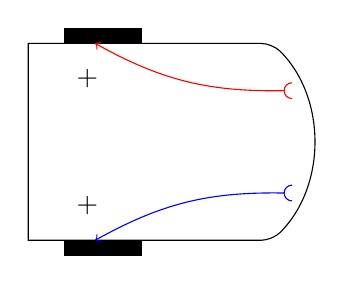
\begin{tikzpicture}[scale=.5]
% Draw big robot
\draw (-2.2cm,-2.5cm) to [rounded corners] (4cm,-2.5cm) to [rounded corners, bend right=45] (4cm,2.5cm) to (-2.2cm,2.5cm) to cycle;
\fill (-1.3cm,-2.5cm) rectangle +(2cm, -.4cm);
\fill (-1.3cm,2.5cm) rectangle +(2cm, .4cm);
\coordinate (right-wheel) at (-.5,-2.5);
\coordinate (left-wheel) at (-.5,2.5);
\node[below,xshift=-1mm,yshift=-2mm] at (left-wheel) {$+$};
\node[above,xshift=-1mm,yshift=2mm] at (right-wheel) {$+$};
% Left sensor and arrows
\coordinate (left-sensor) at (4.3,1.3);
\draw[red] (4.5, 1.5) arc[start angle=90, end angle=270, radius=.2cm];
\draw[->,red] (left-sensor) to [bend left=15] (left-wheel);
% Right sensor and arrows
\coordinate (right-sensor) at (4.3,-1.3);
\draw[blue] (4.5, -1.5) arc[start angle=270, end angle=90, radius=.2cm];
\draw[->,blue] (right-sensor) to [bend right=15] (right-wheel);
\end{tikzpicture}
\caption{Véhicule lâche}\label{fig.coward}
\end{minipage}
\hspace{\fill}
\begin{minipage}{.45\textwidth}
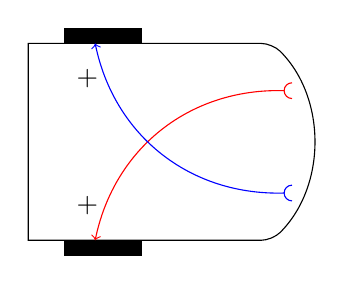
\begin{tikzpicture}[scale=.5]
% Draw big robot
\draw (-2.2cm,-2.5cm) to [rounded corners] (4cm,-2.5cm) to%
[rounded corners, bend right=45] (4cm,2.5cm) to (-2.2cm,2.5cm) to cycle;
\fill (-1.3cm,-2.5cm) rectangle +(2cm, -.4cm);
\fill (-1.3cm,2.5cm) rectangle +(2cm, .4cm);
\coordinate (right-wheel) at (-.5,-2.5);
\coordinate (left-wheel) at (-.5,2.5);
\node[below,xshift=-1mm,yshift=-2mm] at (left-wheel) {$+$};
\node[above,xshift=-1mm,yshift=2mm] at (right-wheel) {$+$};
% Left sensor and arrows
\coordinate (left-sensor) at (4.3,1.3);
\draw[red] (4.5, 1.5) arc[start angle=90, end angle=270, radius=.2cm];
\draw[->,red] (left-sensor) to [bend right=40] (right-wheel);
% Right sensor and arrows
\coordinate (right-sensor) at (4.3,-1.3);
\draw[blue] (4.5, -1.5) arc[start angle=270, end angle=90, radius=.2cm];
\draw[->,blue] (right-sensor) to [bend left=40] (left-wheel);
\end{tikzpicture}
\caption{Véhicule agressif}\label{fig.aggressive}
\end{minipage}
\end{figure}

\begin{framed}
\act{La présentation des véhicules par Braitenberg}{brait-vehicles}
\begin{itemize}
\item Mettre en place les véhicules \emph{coward} et \emph{aggressive}.
\item Utilisez des capteurs de proximité à la place des capteurs de lumière de Braitenberg et la détection ou la non-détection d'un objet à la place de sources lumineuses plus ou moins fortes.
\item Les robots des Figs.~\ref{fig.loves}--\ref{fig.explorer} sont les mêmes que les robots des Figs.~\ref{fig.coward}--\ref{fig.aggressive}, respectivement, sauf que les valeurs des capteurs sont négatives (les signes $-$ sur les connexions) : plus la lumière est détectée, plus la roue tourne lentement. Supposons qu'un biais fixe soit appliqué aux moteurs afin que les roues tournent vers l'avant lorsqu'aucune source de lumière n'est détectée.
\item Implémentez le robot de la Fig.~\ref{fig.loves}. Pourquoi s'appelle-t-il \emph{loves} ?
\item Implémentez le robot de la Fig.~\ref{fig.explorer}. Pourquoi s'appelle-t-il \emph{explorer} ?
\end{itemize}
\end{framed}


\begin{figure}
\begin{minipage}{.45\textwidth}
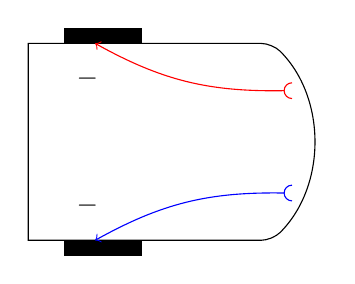
\begin{tikzpicture}[scale=.5]
% Draw big robot
\draw (-2.2cm,-2.5cm) to [rounded corners] (4cm,-2.5cm) to%
[rounded corners, bend right=45] (4cm,2.5cm) to (-2.2cm,2.5cm) to cycle;
\fill (-1.3cm,-2.5cm) rectangle +(2cm, -.4cm);
\fill (-1.3cm,2.5cm) rectangle +(2cm, .4cm);
\coordinate (right-wheel) at (-.5,-2.5);
\coordinate (left-wheel) at (-.5,2.5);
\node[below,xshift=-1mm,yshift=-2mm] at (left-wheel) {$-$};
\node[above,xshift=-1mm,yshift=2mm] at (right-wheel) {$-$};
% Left sensor and arrows
\coordinate (left-sensor) at (4.3,1.3);
\draw[red] (4.5, 1.5) arc[start angle=90, end angle=270, radius=.2cm];
\draw[->,red] (left-sensor) to [bend left=15] (left-wheel);
% Right sensor and arrows
\coordinate (right-sensor) at (4.3,-1.3);
\draw[blue] (4.5, -1.5) arc[start angle=270, end angle=90, radius=.2cm];
\draw[->,blue] (right-sensor) to [bend right=15] (right-wheel);
\end{tikzpicture}
\caption{Véhicule d'amour}\label{fig.loves}
\end{minipage}
\hspace{\fill}
\begin{minipage}{.45\textwidth}
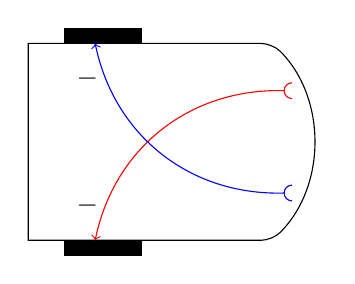
\begin{tikzpicture}[scale=.5]
% Draw big robot
\draw (-2.2cm,-2.5cm) to [rounded corners] (4cm,-2.5cm) to%
[rounded corners, bend right=45] (4cm,2.5cm) to (-2.2cm,2.5cm) to cycle;
\fill (-1.3cm,-2.5cm) rectangle +(2cm, -.4cm);
\fill (-1.3cm,2.5cm) rectangle +(2cm, .4cm);
\coordinate (right-wheel) at (-.5,-2.5);
\coordinate (left-wheel) at (-.5,2.5);
\node[below,xshift=-1mm,yshift=-2mm] at (left-wheel) {$-$};
\node[above,xshift=-1mm,yshift=2mm] at (right-wheel) {$-$};
% Left sensor and arrows
\coordinate (left-sensor) at (4.3,1.3);
\draw[red] (4.5, 1.5) arc[start angle=90, end angle=270, radius=.2cm];
\draw[->,red] (left-sensor) to [bend right=40] (right-wheel);
% Right sensor and arrows
\coordinate (right-sensor) at (4.3,-1.3);
\draw[blue] (4.5, -1.5) arc[start angle=270, end angle=90, radius=.2cm];
\draw[->,blue] (right-sensor) to [bend left=40] (left-wheel);
\end{tikzpicture}
\caption{Véhicule d'exploration}\label{fig.explorer}
\end{minipage}
\end{figure}

\section{Résumé}

Un robot présente un comportement réactif lorsque ses actions dépendent uniquement des valeurs actuelles renvoyées par ses capteurs. Ce chapitre a présenté deux familles de comportement réactif. Les véhicules de Braitenberg mettent en oeuvre un comportement réactif en modifiant le réglage des moteurs en réponse à la détection ou à la non-détection par les capteurs de proximité d'un objet situé à une certaine position par rapport au robot. Ces véhicules démontrent qu'un comportement complexe peut résulter d'algorithmes réactifs relativement simples.

Le suivi de lignes est une tâche fondamentale en robotique. En raison des incertitudes liées au mouvement du robot et à son environnement, les robots utilisent des points de repère tels que des lignes pour s'assurer qu'ils se déplacent vers la destination prévue. Le suivi de ligne est un comportement réactif car le robot modifie son comportement en réponse aux valeurs renvoyées par les capteurs au sol. Nous avons donné trois configurations pour le robot et la ligne, et développé des algorithmes pour chaque cas. La performance des algorithmes dépend des seuils des capteurs et des vitesses des moteurs, qui doivent être déterminés par expérimentation afin de s'assurer que le robot se déplace rapidement tout en restant robuste aux changements de l'environnement.

\section{Autres lectures}

Le livre de Braitenberg \cite{valentino} est intéressant parce qu'il est écrit du point de vue d'un neuroscientifique. Le livre décrit des véhicules utilisant une technologie imaginée, mais ils donnent néanmoins à réfléchir. Les véhicules de Braitenberg décrits ici sont adaptés des implémentations matérielles décrites dans \cite{creatures}. Une implémentation des véhicules de Braitenberg en Scratch par le premier auteur est disponible à l'adresse :
\par\noindent\url{https://scratch.mit.edu/studios/1452106}.
